%%% This thesis template was created by Dr. A. Malkoti (CSIR-NGRI).  
%%% Date: 15 Mar 2018
%%% The template can be used/distributed/modified freely. 
%%% This comes without any gurantee/warantee.
%%% It shouldn't be considered at official format for AcSIR thesis. 


%%%%%%%%%%%%%%%%%%%%%%%%%%%%%%%%%%%%%%%%%%%%%%%%
%%%%%%%%% NGRI Thesis Format %%%%%%%%%%%%%%%%%%

\documentclass[10pt,a4paper]{book}
\usepackage{acsir}
\usepackage{enumitem}


\title{Your Thesis title!}
\docType{Dissertation}  				% default: Thesis
\UnivName{Your Institute Name}			% default: AcSIR

\degreeName{Master in science} 			% default: Doctor of Philosophy
\degreeStream{EARTH SCIENCES}    	  	% default: Physical Sciences
\degreeMajor{(Geology)}				  	% default: Geophysics
%%
\author{YOUR NAME HERE}					% default: blank
\enrolmentNumber{10PP13JXXXX}			% default: blank
\supervisor{Prof. Name}				
\labName{Mention your department here}	% default: CSIR-NGRI
\labAddress{ The addres of Lab}			% default: Hyderabad-500007, India
\theDate{15 Mar 2022}					% default: compiling date 
\instLogo{logo_ngri.png}               	% default: AcSIR Logo


\begin{document}
	\frontmatter 
	\pagestyle{empty}
	
	\maketitle 
	\makecertificate{} 
	% \makeDedication{This is optional.} 
	% \makeAcknowledgement{This is optional} 
	\tableofcontents 
	\listoffigures 
	\listoftables 
	
	
	\chapter*{Summary}
\vspace*{-3em}



Summary of the work 








					% require editing
	\mainmatter 
	\pagestyle{fancy} 
	%
	\chapter{Introduction}

Here first we will show some example for citing the litrature. 
All information is contained in the \textit{mybibfile.bib} file stored in the 
directory \textbf{bibliography}. 


There are two modes for referencing in-text and panrantheis. 
Here is how to reference to in-text  \cite{malkoti_algorithm_2018} or in this way 
in paranthesis \citep{li_matlab_2020}.   
%
You may have it in different modes, which is presented in a form of table as follows


\begin{table}
\caption{Table showing different citation styles}
\label{tab:citation_style}
\begin{tabular}{ll}	
	\hline
	Command  & Effect \\
	\hline
	\verb|\cite{malkoti_algorithm_2018}|   &\cite{malkoti_algorithm_2018}\\
	\verb|\citep{malkoti_algorithm_2018,li_matlab_2020}|   &\citep{malkoti_algorithm_2018,li_matlab_2020}\\
	\verb|\citep[etc.]{malkoti_algorithm_2018,li_matlab_2020}|   &\citep[etc.]{malkoti_algorithm_2018,li_matlab_2020}\\
	\verb|\citep[e.g.][etc.]{malkoti_algorithm_2018,li_matlab_2020}|   &\citep[e.g.][etc.]{malkoti_algorithm_2018,li_matlab_2020} \\
	\hline	
\end{tabular}

\end{table}


\section{Some Random Text Here After}
\lipsum[1-20]
  				% require editing
	\chapter{Theory}

\section{Background}
When you are preparing the theory part various elements are used for that. A few are discussed in following text. 


\subsection{Equations}
	A simple equation can be written as 
	\begin{align}
		a^2 = b^2 +c ^2     \label{eq:theory_pythagorus}
	\end{align}
	%
	To write above equation the code is 
	\begin{verbatim}
	\begin{align}
	a^2 = b^2 +c ^2     \label{eq:theory_pythagorus}
	\end{align}
	\end{verbatim}
	%	
	This equation can be referred anywhere in the text as following \cref{eq:theory_pythagorus} for which the command is  \verb|\cref{eq:theory_pythagorus}|.


	Very complex equations can also be written using latex easily. 
	Following is an example
	
	\begin{align}
		\nabla \times F = \int_{-\infty}^{t} \lambda K(x) \pdv{s}{x} dx
	\end{align}
	


\subsection{Figures}
	Let us show an example of figure insertion here
	\begin{figure}[!h]
		\center
		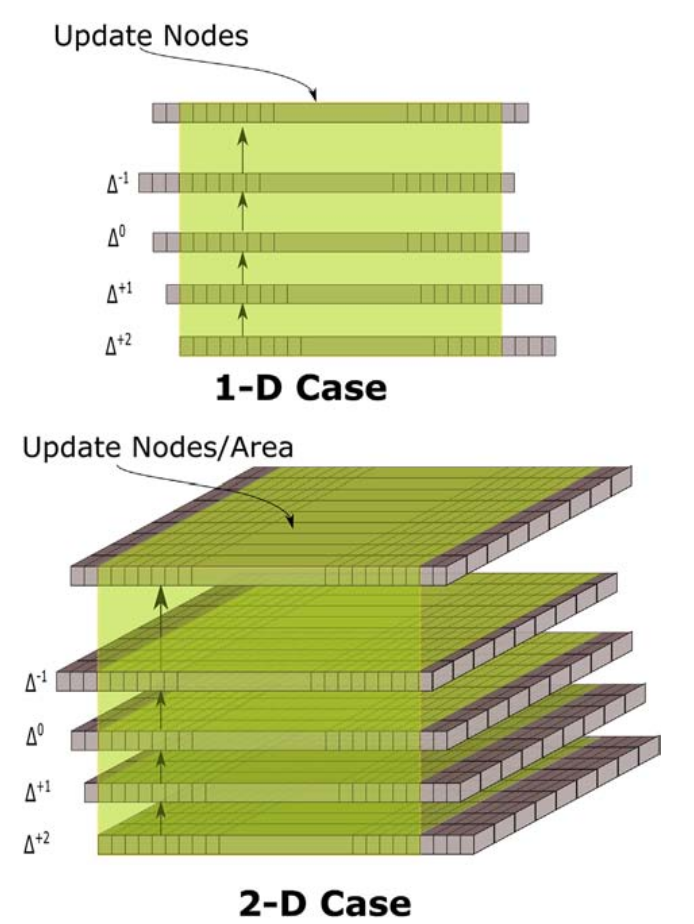
\includegraphics[width=.32\textwidth]{theory_vectorize_operator.png}
		\caption{The figure is taken from  \cite{malkoti_algorithm_2018} 
			to show how to include a figure. 
			A uniquie lable  is attached to this figure so that it can be 
			referred anywhere in the thesis.}
		\label{fig:theory_vectorize}
	\end{figure}

	The code used for inserting the figure is 
	\begin{verbatim}	
	\begin{figure}[!h]
		\center
		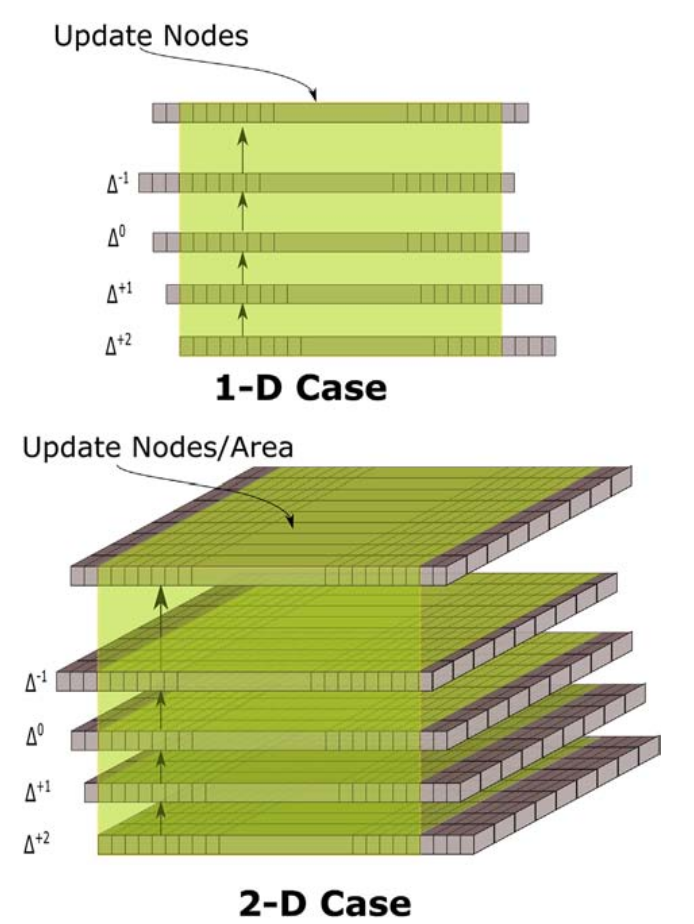
\includegraphics[width=.32\textwidth]{theory_vectorize_operator.png}
		\caption{The figure is taken from  \cite{malkoti_algorithm_2018} to show how 
		to include a figure. A uniquie lable  is attached to this figure so that it 
		can be referred anywhere in the thesis.}
		\label{fig:theory_vectorize}
	\end{figure}
	\end{verbatim}
	
	The figure can be cited anywhere in the text as \cref{fig:theory_vectorize} using the command \verb|\cref{fig:theory_vectorize}|.



\subsection{Tables}
	Now we demonstrate a table which is showing a list of different ways to cite a figure and table.

\begin{table}[!h]
\caption{ List of new commands provided by this package}
\label{tab:list_ref_cmd}
\center
\begin{tabular}{cc}
	\hline
	\verb|\cref{fig:theory_vectorize} |		&	\cref{fig:theory_vectorize}\\
	\verb|\Cref{fig:theory_vectorize}|		&	\Cref{fig:theory_vectorize}\\
	\verb|\cref{tab:citation_style} |		&	\cref{tab:citation_style}\\
	\verb|\Cref{tab:citation_style}|		&	\Cref{tab:citation_style}\\
	\hline
\end{tabular}
\end{table} 


The above table was created using following code
\begin{verbatim}
	\begin{table}[!h]
	\caption{ List of new commands provided by this package}
	\label{tab:list_ref_cmd}
	\center
	\begin{tabular}{cc}
	\hline
	\verb|\cref{fig:theory_vectorize} |		&	\cref{fig:theory_vectorize}\\
	\verb|\Cref{fig:theory_vectorize}|		&	\Cref{fig:theory_vectorize}\\
	\verb|\cref{tab:citation_style} |		&	\cref{tab:citation_style}\\
	\verb|\Cref{tab:citation_style}|		&	\Cref{tab:citation_style}\\
	\hline
	\end{tabular}
	\end{table} 
\end{verbatim}



\subsection{Units}
The units can be correctly formatted as following\\
\begin{tabular}{cc}
	\hline
	                     Command                      &                   Effect                 \\
	                    \hline
	       \verb|1500 \si{\meter\per\second}|         &        1500 \si{\meter\per\second}        \\
	\verb|$ \SI{3.456}{\Newton \per \meter\squared}$| & $ \SI{3.456}{\newton \per \meter\squared}$\\
	\hline
\end{tabular} 

%\section{Some Random Text Here After}
%\lipsum[1-20]

  					% require editing
	\chapter{Results}



\textbf{Some Random Text Here After}
\lipsum[1-20]

  					% require editing
	\chapter{Discussion}

Some random text.\\
Some random text.\\
Some random text.\\
Some random text.\\
Some random text.\\
Some random text.\\
Some random text.\\
Some random text.\\
Some random text.\\
Some random text.\\
Some random text.\\
Some random text.\\
Some random text.\\
Some random text.\\
Some random text.\\
Some random text.\\
Some random text.\\
Some random text.\\
Some random text.\\
Some random text.\\
Some random text.\\
Some random text.\\
Some random text.\\
  				% require editing
	\chapter{Conclusions}

Some random text.\\
Some random text.\\
Some random text.\\
Some random text.\\
Some random text.\\
Some random text.\\
Some random text.\\
Some random text.\\
Some random text.\\
Some random text.\\
Some random text.\\
Some random text.\\
Some random text.\\
Some random text.\\
Some random text.\\
Some random text.\\
Some random text.\\
Some random text.\\
Some random text.\\
Some random text.\\
Some random text.\\
Some random text.\\
Some random text.\\
Some random text.\\
Some random text.\\
Some random text.\\
Some random text.\\
Some random text.\\
Some random text.\\
Some random text.\\
  				% require editing
	
	%% Adding more chapters 
	%% step 1: Create a tex file (e.g FileName.tex) in the directory "chapters" 
	%% step 2: Add here command "\include{chapters/FileName}". 
	
	\appendix
	\chapter{Background details of some method}

\lipsum[1-10]


  \begin{align}
  	a= b
  \end{align}				% require editing
	\chapter{Background details of some other method}


\textbf{Some Random Text Here After}
\lipsum[1-20]
				% require editing
	
	This file contains all your references in bibtex form.
	\bibliography{references/mybibfile}					
	
\end{document}